\documentclass[aspectratio=169]{beamer}

% Shared Beamer settings for Applied Machine Learning lectures (UPES).
% Keep this file free of \documentclass to allow reuse via \input.

% Allow lecture sources to use shared theme/assets without copying them into each lecture folder.
% NOTE: These paths are relative to `Unit-xx/Lecture-yy/latex/` (and `Lab/Experiment-xx/latex/`).
\makeatletter
\def\input@path{{../../../_shared/}{../../../_shared/UPES-Beamer-Theme/}}
\makeatother

\usetheme{UPES}
\setbeamertemplate{navigation symbols}{}

\usepackage{amsmath}
\usepackage{amssymb}
\usepackage{booktabs}
\usepackage{graphicx}
\usepackage{hyperref}
\usepackage{xcolor}
\usepackage{listings}

% Code listings (Python-oriented for this subject).
\lstset{
  language=Python,
  basicstyle=\ttfamily\small,
  keywordstyle=\color{blue},
  commentstyle=\color{gray},
  stringstyle=\color{teal},
  showstringspaces=false,
  columns=fullflexible,
  breaklines=true
}

\usepackage{tikz}
\usetikzlibrary{arrows.meta,positioning,shapes.geometric,calc,fit,backgrounds}

% Per-slide source line (references shown on the slide itself).
\newcommand{\slidesources}[1]{%
  \vfill
  {\tiny\color{gray}\raggedright\sloppy\parbox{\linewidth}{Sources: #1}\par}%
}

% Unit-wise source strings for this subject (used by slides/notes).
% Path is relative to the lecture `latex/` folder (the compilation CWD).
% Source strings for Applied Machine Learning (CSAI2017P) — used by slides + notes.
% Prescribed texts and reference books are taken from the course syllabus.
% Support texts are the author-hosted open-access editions:
%   statlearning.com            (ISL with Python)
%   probml.github.io/pml-book   (Murphy, Probabilistic Machine Learning)
%   d2l.ai                      (Dive into Deep Learning)
%   mml-book.github.io          (Mathematics for Machine Learning)

\newcommand{\AMLRepoURL}{https://github.com/tali7c/Applied-Machine-Learning}

% --- prescribed -------------------------------------------------------------
\newcommand{\AMLPrescribed}{%
M\"uller and Guido, \textit{Introduction to Machine Learning with Python}, O'Reilly, 2016.;%
Bishop, \textit{Pattern Recognition and Machine Learning}, Springer, 2006.;%
Murphy, \textit{Machine Learning: A Probabilistic Perspective}, MIT Press, 2012.;%
Han, Kamber and Pei, \textit{Data Mining: Concepts and Techniques} (3e), Morgan Kaufmann, 2012.%
}

% --- unit-wise ---------------------------------------------------------------
\newcommand{\AMLUnitISources}{%
M\"uller and Guido, \textit{Introduction to Machine Learning with Python}, Ch. 1.;%
Bishop, \textit{Pattern Recognition and Machine Learning}, Ch. 1.;%
Murphy, \textit{Probabilistic Machine Learning: An Introduction}, MIT Press, 2022, Ch. 1.;%
Mitchell, \textit{Machine Learning}, McGraw Hill, 1997, Ch. 1.;%
Scikit-learn documentation, accessed 2026-08-04.%
}

\newcommand{\AMLUnitIISources}{%
Bishop, \textit{Pattern Recognition and Machine Learning}, \S1.5, \S4.3, \S7.1.;%
Zhang, Lipton, Li and Smola, \textit{Dive into Deep Learning}, \S3.4.;%
Shalev-Shwartz and Ben-David, \textit{Understanding Machine Learning}, Ch. 15.;%
Murphy, \textit{Probabilistic Machine Learning: An Introduction}, Ch. 5.%
}

\newcommand{\AMLUnitIIISources}{%
Zhang, Lipton, Li and Smola, \textit{Dive into Deep Learning}, Ch. 12 (Optimization Algorithms).;%
Deisenroth, Faisal and Ong, \textit{Mathematics for Machine Learning}, Ch. 7.;%
Kingma and Ba, ``Adam: A Method for Stochastic Optimization,'' ICLR 2015.;%
Ruder, ``An overview of gradient descent optimization algorithms,'' arXiv:1609.04747, 2016.%
}

\newcommand{\AMLUnitIVSources}{%
Han, Kamber and Pei, \textit{Data Mining: Concepts and Techniques} (3e), Ch. 3.;%
M\"uller and Guido, \textit{Introduction to Machine Learning with Python}, Ch. 3--4.;%
James, Witten, Hastie, Tibshirani and Taylor, \textit{An Introduction to Statistical Learning with Python}, Ch. 5--6, 12.;%
Scikit-learn documentation (preprocessing, model selection), accessed 2026-08-04.%
}

\newcommand{\AMLUnitVSources}{%
James et al., \textit{An Introduction to Statistical Learning with Python}, Ch. 3--6.;%
Bishop, \textit{Pattern Recognition and Machine Learning}, Ch. 3.;%
Deisenroth, Faisal and Ong, \textit{Mathematics for Machine Learning}, Ch. 9.;%
M\"uller and Guido, \textit{Introduction to Machine Learning with Python}, \S2.3.%
}

\newcommand{\AMLUnitVISources}{%
Han, Kamber and Pei, \textit{Data Mining: Concepts and Techniques} (3e), Ch. 8--9.;%
James et al., \textit{An Introduction to Statistical Learning with Python}, Ch. 8--9.;%
Bishop, \textit{Pattern Recognition and Machine Learning}, Ch. 4--5, 7, 14.;%
Zhang et al., \textit{Dive into Deep Learning}, Ch. 5.%
}

\newcommand{\AMLUnitVIISources}{%
Han, Kamber and Pei, \textit{Data Mining: Concepts and Techniques} (3e), Ch. 10.;%
James et al., \textit{An Introduction to Statistical Learning with Python}, Ch. 12.;%
M\"uller and Guido, \textit{Introduction to Machine Learning with Python}, \S3.5.;%
Ester, Kriegel, Sander and Xu, ``A density-based algorithm for discovering clusters (DBSCAN),'' KDD 1996.%
}

\newcommand{\AMLLabSources}{%
M\"uller and Guido, \textit{Introduction to Machine Learning with Python}, companion notebooks.;%
McKinney, \textit{Python for Data Analysis} (3e), O'Reilly, 2022.;%
Scikit-learn user guide, accessed 2026-08-04.;%
Matplotlib and Seaborn documentation, accessed 2026-08-04.%
}



\graphicspath{{../figures/}{../images/}{../../../_shared/}{../../../_shared/UPES-Beamer-Theme/}}

\title[Applied Machine Learning]{Applied Machine Learning}
\subtitle{Unit 02 -- Lecture 02: Loss Functions}
\author{Tofik Ali}
\institute{School of Computer Science, UPES Dehradun}
\date{Autumn 2026}

% ---- a compact "output" block so code and its result sit together ----------
\lstdefinestyle{outblk}{
  basicstyle=\ttfamily\scriptsize\color{black!75},
  backgroundcolor=\color{black!5}, frame=leftline, framerule=2pt,
  rulecolor=\color{black!30}, breaklines=true, columns=fullflexible,
  keepspaces=true,   % several outputs below are aligned tables
  language={},       % printed output is not Python: do not syntax-highlight it
  xleftmargin=4pt, aboveskip=1pt, belowskip=1pt, literate={-}{{-}}1}
\lstnewenvironment{outblk}{\lstset{style=outblk}}{}

\begin{document}

\UPESCoverFrame
\setcounter{framenumber}{0}

\begin{frame}
  \titlepage
  \vspace{0.3em}
  \begin{center}
    \footnotesize Topic focus: \textbf{what number are we trying to make small?}\\[0.25em]
    \footnotesize Repository: \texttt{\AMLRepoURL}
  \end{center}
  \slidesources{\AMLUnitIISources}
\end{frame}

\begin{frame}{Quick Links}
  \centering
  \hyperlink{sec:what}{\beamerbutton{What a loss is}}\hspace{0.5em}
  \hyperlink{sec:reg}{\beamerbutton{Regression}}\hspace{0.5em}
  \hyperlink{sec:clf}{\beamerbutton{Classification}}\hspace{0.5em}
  \hyperlink{sec:margin}{\beamerbutton{Margins}}\hspace{0.5em}
  \hyperlink{sec:choose}{\beamerbutton{Choosing}}\hspace{0.5em}
  \hyperlink{sec:summary}{\beamerbutton{Summary}}
\end{frame}

\begin{frame}{Agenda}
  \tableofcontents
\end{frame}

\begin{frame}{How this lecture works}
  \begin{columns}[T]
    \begin{column}{0.48\textwidth}
      \begin{block}{Every idea appears twice}
        \begin{enumerate}
          \item \textbf{By hand} --- small numbers, on paper, so you see the
            mechanism.
          \item \textbf{In code} --- the same thing, so you see the library does
            exactly that and nothing magic.
        \end{enumerate}
      \end{block}
    \end{column}
    \begin{column}{0.48\textwidth}
      \begin{alertblock}{Commit before you look}
        Four slides ask you to predict an answer before it is revealed. Write
        your guess down. Being wrong on paper is how the idea sticks.
      \end{alertblock}
    \end{column}
  \end{columns}
  \vspace{0.4em}
  \begin{center}
    \small Full derivations, more worked examples and 10 practice questions
    with solutions are in \texttt{notes.pdf}.
  \end{center}
\end{frame}

\begin{frame}[shrink=6]{No Dataset, No Seed}
  \begin{block}{The reproducibility convention, and why today is the exception}
    \small
    \begin{itemize}
      \item Every other lecture fixes \textbf{one dataset and one seed}, always
        shown in the listing --- the convention from Lecture~1.
      \item A loss function is arithmetic on numbers you already have. It does
        not sample, shuffle or initialise.
      \item So today there is \textbf{no dataset and no random number at all}:
        four house prices, three emails, six sensor readings, written out.
    \end{itemize}
  \end{block}
  \begin{alertblock}{What that buys you}
    \small Every value in these slides is not just reproducible but
    \emph{inevitable}. Run a listing and get something else, and it is a typing
    mistake --- chance never got a turn. Randomness returns in Lecture~3, and
    with it \texttt{np.random.default\_rng(0)} on every listing that needs one.
  \end{alertblock}
\end{frame}

\begin{frame}{Where we are}
  \begin{columns}[T]
    \begin{column}{0.46\textwidth}
      \begin{block}{Unit I gave us}
        The shape of the problem: data, a model family, and the need to
        generalise.
      \end{block}
      \begin{exampleblock}{Unit II (today)}
        \textbf{What} quantity do we minimise?
      \end{exampleblock}
      \begin{block}{Unit III (next)}
        \textbf{How} do we minimise it?
      \end{block}
    \end{column}
    \begin{column}{0.5\textwidth}
      \begin{alertblock}{Why this order}
        Once you know what is being minimised and how the minimising is done,
        every method in Units V--VII is a variation on one theme rather than a
        new thing to memorise.
      \end{alertblock}
    \end{column}
  \end{columns}
\end{frame}

% =====================================================================
\section{What a loss function is}
\label{sec:what}

\begin{frame}{Fitting any supervised model: three steps}
  \begin{enumerate}
    \item<1-> Propose a family of candidate models, controlled by parameters.
    \item<2-> Define \textbf{one number} saying how badly a candidate does.
    \item<3-> Search the parameters to make that number small.
  \end{enumerate}
  \vspace{0.8em}
  \onslide<4->{
  \begin{exampleblock}{Step 2 is the loss function}
    That is this entire lecture. Step 3 is Unit III.
  \end{exampleblock}}
  \vspace{0.4em}
  \onslide<5->{
  \begin{alertblock}{The compression is where the judgement lives}
    A loss turns \emph{a set of mistakes} into \emph{one number}. By choosing
    how, you declare what kind of mistake you consider serious.
  \end{alertblock}}
\end{frame}

\begin{frame}{Three words that are not synonyms}
  \begin{center}
  \small
  \begin{tabular}{@{}lp{7.6cm}@{}}
    \toprule
    \textbf{Loss} & computed on \emph{one} example\\[3pt]
    \textbf{Cost} / objective & the loss averaged over the training set,
      plus regularization --- the thing actually minimised\\[3pt]
    \textbf{Metric} & what you \emph{report} to a human; need not be
      differentiable, need not be what you optimised\\
    \bottomrule
  \end{tabular}
  \end{center}
  \vspace{0.5em}
  \begin{alertblock}{The loss and the metric are allowed to differ}
    Train with cross-entropy, report F1. Train with Huber, report RMSE.
    That is normal. What is \emph{not} acceptable is failing to notice when
    they disagree about which model is better.
  \end{alertblock}
\end{frame}

\begin{frame}{A loss must satisfy two things}
  \begin{columns}[T]
    \begin{column}{0.47\textwidth}
      \begin{block}{1. Small when the model is right}
        Obvious --- and it rules out less than you would think.
      \end{block}
    \end{column}
    \begin{column}{0.47\textwidth}
      \begin{block}{2. Usable by the optimiser}
        Differentiable almost everywhere, with a gradient that points
        somewhere useful.
      \end{block}
    \end{column}
  \end{columns}
  \vspace{1em}
  \begin{center}
    \textbf{Requirement 2 is why we cannot optimise the thing we actually
    care about.}\\[0.3em]
    \small We come back to this in the classification section.
  \end{center}
\end{frame}

% =====================================================================
\section{Regression losses}
\label{sec:reg}

\begin{frame}{The residual is the raw material}
  \begin{center}
    \Large $r_i \;=\; y_i - \hat{y}_i$
  \end{center}
  \vspace{0.6em}
  Every regression loss is a rule for turning a residual into a non-negative
  penalty, then averaging.
  \vspace{0.8em}
  \begin{center}
  \begin{tabular}{@{}lll@{}}
    \toprule
    \textbf{MSE}  & $\frac{1}{n}\sum r_i^2$          & squaring: twice as wrong costs \emph{four} times\\[3pt]
    \textbf{MAE}  & $\frac{1}{n}\sum |r_i|$          & absolute: twice as wrong costs \emph{twice}\\[3pt]
    \textbf{RMSE} & $\sqrt{\mathrm{MSE}}$            & same model as MSE --- exists for \emph{reporting}\\
    \bottomrule
  \end{tabular}
  \end{center}
  \vspace{0.4em}
  \begin{center}\small
    RMSE is not a separate loss: the square root is increasing, so it gives the
    \emph{identical} model. It exists so the number can be read aloud.
  \end{center}
\end{frame}

\begin{frame}{By hand: four houses}
  \begin{center}
  \begin{tabular}{@{}lrrrr@{}}
    \toprule
    $y$ (lakhs)      & 3.0 & 5.0 & 2.0 & 8.0\\
    $\hat{y}$        & 2.5 & 5.5 & 4.0 & 7.0\\
    \midrule
    $r$              & 0.5 & $-0.5$ & $-2.0$ & 1.0\\
    $r^2$            & 0.25 & 0.25 & \textbf{4.0} & 1.0\\
    $|r|$            & 0.5 & 0.5 & \textbf{2.0} & 1.0\\
    \bottomrule
  \end{tabular}
  \end{center}
  \vspace{0.3em}
  \begin{center}
    $\mathrm{MSE}=\frac{5.5}{4}=1.375$ \qquad
    $\mathrm{MAE}=\frac{4}{4}=1.0$ \qquad
    $\mathrm{RMSE}=\sqrt{1.375}=1.173$
  \end{center}
  \vspace{0.2em}
  \begin{alertblock}{Look at the third house}
    \small It contributes \textbf{4 of the 5.5} squared-error total --- 73\% of
    the loss from 25\% of the data. Under MAE: 2 of 4, exactly half.
  \end{alertblock}
\end{frame}

\begin{frame}[fragile]{The same thing in code}
\begin{lstlisting}
import numpy as np
from sklearn.metrics import mean_squared_error, mean_absolute_error

y    = np.array([3.0, 5.0, 2.0, 8.0])
yhat = np.array([2.5, 5.5, 4.0, 7.0])
r = y - yhat

print("MSE  np     ", np.mean(r**2))
print("MAE  np     ", np.mean(np.abs(r)))
print("MSE  sklearn", mean_squared_error(y, yhat))
\end{lstlisting}
\begin{outblk}
MSE  np      1.375
MAE  np      1.0
MSE  sklearn 1.375
\end{outblk}
\end{frame}

\begin{frame}[shrink=4]{What each loss charges}
  \begin{center}
    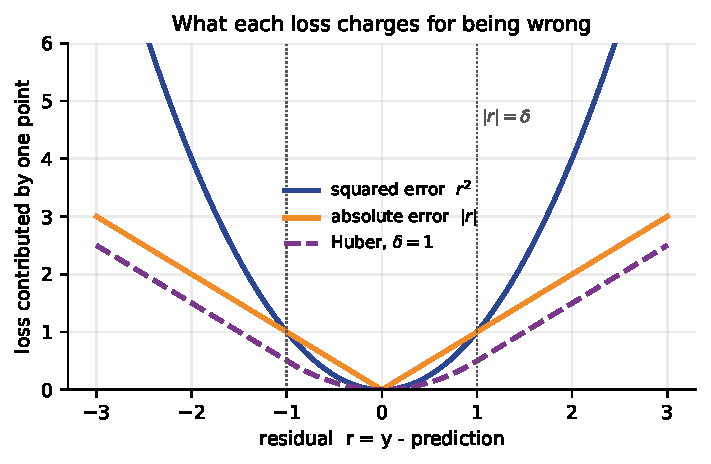
\includegraphics[width=0.60\textwidth]{losscurves.pdf}
  \end{center}
  \begin{center}\small
    A bowl, a V with a kink at zero, and Huber --- bowl near zero, V far away.
  \end{center}
\end{frame}

\begin{frame}{Predict first \#1}
  \begin{exampleblock}{Six readings, and you must predict one constant}
    \begin{center}
      \texttt{[10, 11, 12, 13, 14, 14]}
    \end{center}
    A sensor now corrupts the last one: \texttt{14} becomes \texttt{94}.
  \end{exampleblock}
  \begin{center}
    \textbf{What happens to the best constant under MSE?  Under MAE?}
  \end{center}
  \vspace{0.3em}
  \onslide<2->{
  \begin{center}
  \begin{tabular}{@{}lrr@{}}
    \toprule
    & \textbf{best under MSE} & \textbf{best under MAE}\\
    \midrule
    clean        & 12.33 & 12.50\\
    with outlier & \textbf{25.67} & \textbf{12.50}\\
    \bottomrule
  \end{tabular}
  \end{center}}
  \onslide<3->{\begin{center}\small
    The MSE answer moved \emph{past every clean observation}. MAE did not move.
  \end{center}}
\end{frame}

\begin{frame}[shrink=9]{Why: MSE fits the mean, MAE fits the median}
  \begin{columns}[T]
    \begin{column}{0.44\textwidth}
      \begin{block}{Minimising $\sum (y_i-c)^2$}
        gives $c = \bar{y}$, the \textbf{mean}
      \end{block}
      \begin{block}{Minimising $\sum |y_i-c|$}
        gives $c = \mathrm{median}(y)$
      \end{block}
      \vspace{0.2em}
      \small Both proofs are in the notes.
    \end{column}
    \begin{column}{0.54\textwidth}
      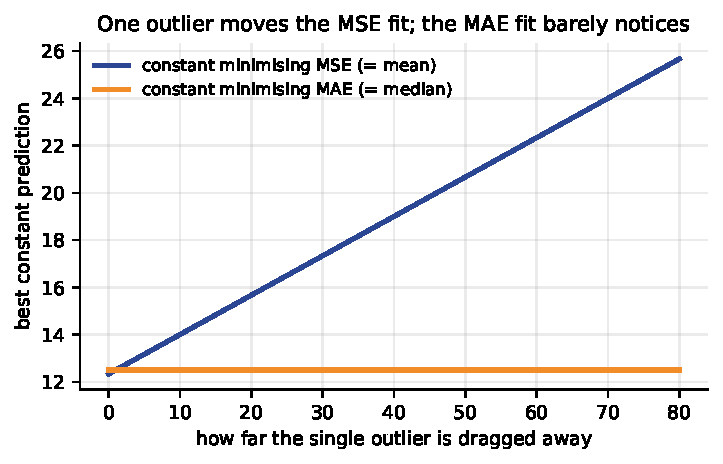
\includegraphics[width=\textwidth]{outlier.pdf}
    \end{column}
  \end{columns}
  \begin{alertblock}{The sentence to remember}
    \small Choosing a loss is not choosing how to \emph{score} your model. It is
    choosing \textbf{what your model will become}.
  \end{alertblock}
\end{frame}

\begin{frame}[fragile]{Confirming it numerically}
\begin{lstlisting}
outlier = np.array([10., 11., 12., 13., 14., 94.])
grid = np.linspace(0, 100, 200001)
mse = ((outlier[:,None] - grid[None,:])**2).mean(axis=0)
mae = (np.abs(outlier[:,None] - grid[None,:])).mean(axis=0)
print("argmin MSE ->", round(grid[mse.argmin()], 4))
print("argmin MAE ->", round(grid[mae.argmin()], 4))
\end{lstlisting}
\begin{outblk}
argmin MSE -> 25.6665
argmin MAE -> 12.0
\end{outblk}
\onslide<2->
\begin{alertblock}{Why 12.0 and not the median 12.5?}
  \footnotesize With an \emph{even} sample the MAE is \textbf{flat} across
  $[12,13]$ --- every constant there is equally optimal, and \texttt{argmin}
  returns the first. A flat loss means \textbf{zero gradient}: that is why MAE
  is harder to optimise than MSE.
\end{alertblock}
\end{frame}

\begin{frame}{Huber: take the good half of each}
  \[
    L_\delta(r)=
    \begin{cases}
      \tfrac{1}{2}r^2, & |r| \le \delta\\[4pt]
      \delta\left(|r|-\tfrac{1}{2}\delta\right), & |r| > \delta
    \end{cases}
  \]
  \vspace{0.2em}
  \begin{columns}[T]
    \begin{column}{0.5\textwidth}
      \begin{block}{The pieces meet smoothly}
        The linear branch is the tangent to the quadratic at $r=\delta$, so
        value \emph{and} slope match. Differentiable everywhere.
      \end{block}
    \end{column}
    \begin{column}{0.46\textwidth}
      \begin{alertblock}{$\delta$ carries the units of $y$}
        $\delta = 1$ means something different for prices in lakhs than for
        temperatures. Set it by cross-validation --- never copy it from a
        tutorial.
      \end{alertblock}
    \end{column}
  \end{columns}
\end{frame}

\begin{frame}{By hand, then in code: Huber with $\delta=1$}
  Same four residuals: $0.5,\ -0.5,\ -2.0,\ 1.0$
  \begin{center}\small
  \begin{tabular}{@{}lll@{}}
    \toprule
    $|0.5| \le 1$   & quadratic & $\tfrac12(0.5)^2 = 0.125$\\
    $|-0.5| \le 1$  & quadratic & $0.125$\\
    $|-2.0| > 1$    & \textbf{linear} & $1\cdot(2-0.5) = 1.5$\\
    $|1.0| \le 1$   & quadratic & $\tfrac12(1)^2 = 0.5$\\
    \midrule
    \multicolumn{2}{@{}l}{mean} & $2.25/4 = \mathbf{0.5625}$\\
    \bottomrule
  \end{tabular}
  \end{center}
  \vspace{0.4em}
  \begin{center}\small
    Squared error charged that third point \textbf{4.0}. Huber charged it
    \textbf{1.5}.
  \end{center}
\end{frame}

\begin{frame}[fragile]{Huber in code}
\begin{lstlisting}
def huber(r, d=1.0):
    a = np.abs(r)
    return np.where(a <= d, 0.5*r**2, d*(a - 0.5*d))

print("per point", huber(r, 1.0))
print("mean     ", huber(r, 1.0).mean())
\end{lstlisting}
\begin{outblk}
per point [0.125 0.125 1.5   0.5  ]
mean      0.5625
\end{outblk}
\begin{center}\small
  $\delta$ larger than every residual $\Rightarrow$ you have chosen scaled MSE.
\end{center}
\end{frame}

% =====================================================================
\section{Classification losses}
\label{sec:clf}

\begin{frame}{The obvious loss, and why it fails}
  \begin{center}
    Charge \textbf{1} for a wrong answer, \textbf{0} for a right one.\\[0.3em]
    This is the \textbf{0--1 loss} --- exactly what accuracy measures.
  \end{center}
  \vspace{1em}
  \begin{center}
    \Large It is also almost useless for \emph{training}.
  \end{center}
  \vspace{1em}
  \begin{center}\small
    The next slide asks you to see why before I say it.
  \end{center}
\end{frame}

\begin{frame}[fragile]{Predict first \#2}
A one-parameter classifier predicts class 1 when $wx>0$. Four points,
two per class. We sweep $w$.

\begin{center}
  \textbf{How many distinct values can accuracy take?
  Can it tell $w{=}1$ from $w{=}2$?}
\end{center}
\vspace{0.4em}
\onslide<2->
\begin{outblk}
w= -2.0  accuracy=0.00  log-loss=3.0725
w= -1.0  accuracy=0.00  log-loss=1.7201
w=  0.0  accuracy=0.50  log-loss=0.6931
w=  1.0  accuracy=1.00  log-loss=0.2201
w=  2.0  accuracy=1.00  log-loss=0.0725
\end{outblk}
\onslide<3->
\begin{alertblock}{Three values. And no, it cannot.}
  \small Accuracy is a \textbf{step function}: flat everywhere, derivative
  zero. Gradient descent standing on it is told ``every direction is equally
  good''. Cross-entropy falls strictly the whole way.
\end{alertblock}
\end{frame}

\begin{frame}{Surrogate losses}
  \begin{exampleblock}{The move that makes classification trainable}
    We optimise a \textbf{surrogate} --- a smooth loss that stands in for the
    thing we actually care about.
  \end{exampleblock}
  \vspace{0.6em}
  \begin{center}
  \begin{tabular}{@{}ll@{}}
    \toprule
    \textbf{What we care about} & 0--1 loss (accuracy)\\
    \textbf{What we minimise}   & cross-entropy, or hinge\\
    \bottomrule
  \end{tabular}
  \end{center}
  \vspace{0.8em}
  \begin{center}
    \small This is why the number you optimise and the number you report are
    so often different. Not carelessness --- necessity.
  \end{center}
\end{frame}

\begin{frame}{Binary cross-entropy}
  \[
    \mathrm{BCE} = -\frac{1}{n}\sum_i
      \Big[\, y_i \log p_i + (1-y_i)\log(1-p_i) \,\Big]
  \]
  \vspace{0.2em}
  \begin{alertblock}{The bracket has two terms but only ever contributes one}
    $y_i = 1 \Rightarrow$ second term vanishes.\quad
    $y_i = 0 \Rightarrow$ first term vanishes.
  \end{alertblock}
  \vspace{0.5em}
  \begin{exampleblock}{So the formula says something very simple}
    Take the probability the model gave \textbf{the class that was actually
    correct}. Take its negative logarithm. Average. That is all it is.
  \end{exampleblock}
\end{frame}

\begin{frame}{By hand: three emails}
  \begin{center}
  \begin{tabular}{@{}lrrr@{}}
    \toprule
    true $y$ (1 = spam)     & 1   & 0   & 1\\
    model $p$ (spam)        & 0.9 & 0.2 & 0.4\\
    \midrule
    prob.\ of \emph{correct} class & 0.9 & \textbf{0.8} & 0.4\\
    $-\log(\cdot)$          & 0.1054 & 0.2231 & \textbf{0.9163}\\
    \bottomrule
  \end{tabular}
  \end{center}
  \vspace{0.5em}
  \begin{center}
    \small Row three is the only step with content: email 2's correct class was
    \emph{not} spam, so we take $1-p = 0.8$.
  \end{center}
  \vspace{0.3em}
  \[
    \mathrm{BCE} = \frac{0.1054+0.2231+0.9163}{3} = \mathbf{0.4149}
  \]
  \begin{center}\small
    The third email was not even confidently wrong --- $0.4$ is near a coin
    flip --- and it still cost more than the other two combined.
  \end{center}
\end{frame}

\begin{frame}[fragile]{The same thing in code}
\begin{lstlisting}
from sklearn.metrics import log_loss

y = np.array([1, 0, 1])
p = np.array([0.9, 0.2, 0.4])
pc = np.where(y == 1, p, 1 - p)   # prob given to the correct class

print("prob correct ", pc)
print("BCE by hand  ", (-np.log(pc)).mean())
print("BCE sklearn  ", log_loss(y, p))
\end{lstlisting}
\begin{outblk}
prob correct  [0.9 0.8 0.4]
BCE by hand   0.414931599615397
BCE sklearn   0.414931599615397
\end{outblk}
\end{frame}

\begin{frame}{Predict first \#3}
  \begin{center}
    A model gives probability \textbf{0.99} to the correct class.
    Loss $= 0.0101$.\\[0.6em]
    \textbf{Another gives 0.01 to the correct class. How many times worse?}
  \end{center}
  \vspace{0.8em}
  \onslide<2->{
  \begin{center}\small
  \begin{tabular}{@{}rrl@{}}
    \toprule
    $p$ correct & loss & \\
    \midrule
    0.99  & 0.0101 & confident and right --- nearly free\\
    0.50  & 0.6931 & a coin flip costs $\log 2$\\
    0.01  & \textbf{4.6052} & \textbf{458$\times$} the cost of being right\\
    0.001 & 6.9078 & and it keeps going\\
    \bottomrule
  \end{tabular}
  \end{center}}
  \vspace{0.4em}
  \onslide<3->{\begin{center}\small
    As $p \to 0$ the loss grows \textbf{without bound}. That is the design:
    it forces models to be honest about uncertainty instead of confidently
    guessing.
  \end{center}}
\end{frame}

\begin{frame}[shrink=13]{Confident and wrong}
  \begin{center}
    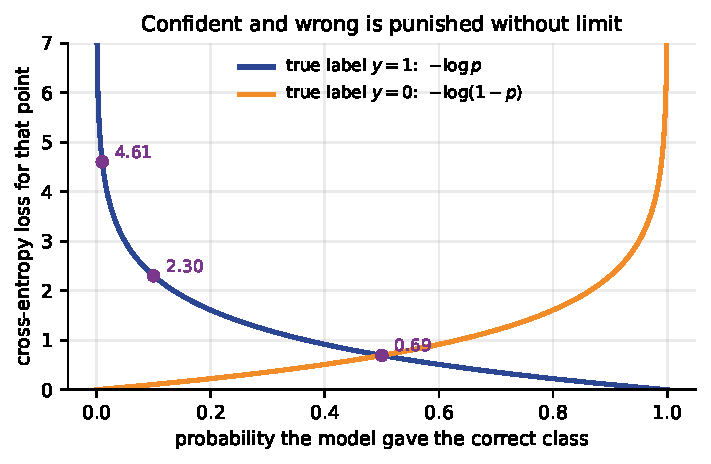
\includegraphics[width=0.55\textwidth]{logloss.pdf}
  \end{center}
  \begin{alertblock}{$\log 0$ is not a number}
    \small Exactly 0 or 1 gives infinite loss and kills the run. Libraries clip
    into $[\varepsilon, 1-\varepsilon]$ --- which is why you feed
    \texttt{log\_loss} \emph{probabilities}, not hard 0/1 predictions.
  \end{alertblock}
\end{frame}

\begin{frame}[fragile]{Categorical vs sparse categorical: the same loss}
\begin{lstlisting}
P = np.array([[0.7,0.2,0.1], [0.1,0.8,0.1], [0.2,0.2,0.6]])
onehot = np.array([[1,0,0], [0,1,0], [0,0,1]])   # categorical
sparse = np.array([0, 1, 2])                      # sparse categorical

print("categorical", -np.sum(onehot*np.log(P), axis=1).mean())
print("sparse     ", -np.log(P[np.arange(3), sparse]).mean())
\end{lstlisting}
\begin{outblk}
categorical 0.3635480396729776
sparse      0.3635480396729776
\end{outblk}
\vspace{0.2em}
\begin{center}\small
  Identical to sixteen decimals --- it is the same arithmetic.
  \textbf{Only the label format differs.}
\end{center}
\end{frame}

\begin{frame}{Why the sparse form exists}
  \begin{exampleblock}{Pure memory economics}
    $K = 10{,}000$ classes, batch of 256.\\[0.3em]
    One-hot: $2.56$ million numbers, of which \textbf{256} are non-zero.\\
    Sparse: \textbf{256 integers}, indexed directly.
  \end{exampleblock}
  \vspace{0.6em}
  \begin{alertblock}{One of the commonest beginner errors}
    Choosing the wrong one in Keras or PyTorch gives an unhelpful error
    message.\\[0.3em]
    \textbf{Check the shape of your labels:} 2-D means categorical, 1-D means
    sparse.
  \end{alertblock}
\end{frame}

% =====================================================================
\section{Margin losses}
\label{sec:margin}

\begin{frame}{When there is no probability to work with}
  An SVM outputs a raw score $f(x)$ --- positive for one class, negative for
  the other. Cross-entropy needs a probability, so we need something else.
  \vspace{0.8em}
  \begin{center}
    Relabel classes as $y \in \{-1, +1\}$ and define the \textbf{margin}\\[0.4em]
    \Large $m_i = y_i \, f(x_i)$
  \end{center}
  \vspace{0.8em}
  \begin{center}
    \small Positive exactly when the prediction is \emph{correct};
    its size says how \emph{decisively}. A margin loss looks at nothing else.
  \end{center}
\end{frame}

\begin{frame}{Hinge loss}
  \begin{center}
    \Large $L_{\mathrm{hinge}}(m) = \max(0,\; 1 - m)$
  \end{center}
  \vspace{0.6em}
  \begin{center}
    Margin at least 1 $\Rightarrow$ loss zero. Otherwise pay the shortfall.
  \end{center}
  \vspace{0.8em}
  \begin{alertblock}{The consequence worth remembering}
    Hinge \textbf{stops caring} once you are right by a comfortable margin.
    Cross-entropy never entirely stops --- it will always take a little more
    confidence.\\[0.4em]
    That is why an SVM is determined by a handful of \emph{support vectors},
    while logistic regression is influenced by every point.
  \end{alertblock}
\end{frame}

\begin{frame}{Predict first \#4}
  \begin{center}
  \begin{tabular}{@{}lrrr@{}}
    \toprule
    true $y$     & $+1$ & $-1$ & $+1$\\
    score $f(x)$ & 2.0  & $-0.5$ & 0.3\\
    \bottomrule
  \end{tabular}
  \end{center}
  \vspace{0.5em}
  \begin{center}
    \textbf{All three are classified correctly. So is the total hinge loss
    zero?}
  \end{center}
  \vspace{0.6em}
  \onslide<2->{
  \begin{center}
  \begin{tabular}{@{}lrrr@{}}
    \toprule
    margin $m = yf$   & 2.0  & 0.5  & 0.3\\
    $\max(0, 1-m)$    & \textbf{0.0}  & 0.5  & 0.7\\
    \bottomrule
  \end{tabular}
  \end{center}
  \vspace{0.3em}
  \begin{center}
    $L = (0.0+0.5+0.7)/3 = \mathbf{0.4}$
  \end{center}}
  \onslide<3->{\begin{center}\small
    Two \emph{correctly classified} points still cost --- they sit inside the
    margin band. That is what produces a \textbf{wide} boundary.
  \end{center}}
\end{frame}

\begin{frame}[fragile]{Hinge in code --- and a floating-point warning}
\begin{lstlisting}
from sklearn.metrics import hinge_loss

ys = np.array([1, -1, 1])
f  = np.array([2.0, -0.5, 0.3])

print("margins      ", ys * f)
print("hinge by hand", np.maximum(0, 1 - ys*f).mean())
print("hinge sklearn", hinge_loss(ys, f))
\end{lstlisting}
\begin{outblk}
margins       [2.  0.5 0.3]
hinge by hand 0.39999999999999997
hinge sklearn 0.39999999999999997
\end{outblk}
\begin{center}\small
  That is $0.4$. Binary floating point cannot represent it exactly --- never
  test loss values with \texttt{==}; use \texttt{np.isclose}.
\end{center}
\end{frame}

\begin{frame}[shrink=4]{The family portrait}
  \begin{center}
    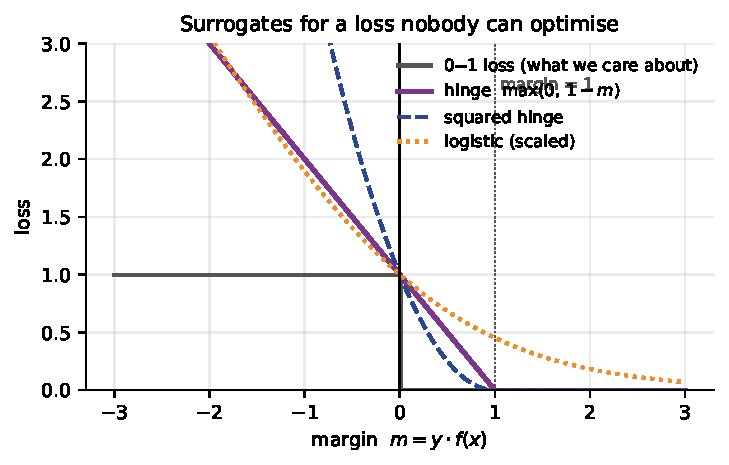
\includegraphics[width=0.54\textwidth]{margin.pdf}
  \end{center}
  \begin{itemize}\footnotesize
    \item Every surrogate sits \textbf{above} the 0--1 step --- that is what
      makes it a legitimate stand-in.
    \item Hinge reaches exactly zero at $m=1$; logistic approaches but never
      arrives.
    \item Left of zero, hinge grows linearly and squared hinge quadratically.
  \end{itemize}
\end{frame}

\begin{frame}[shrink=16]{Triplet loss: a different question entirely}
  \small Sometimes we do not want to classify --- we want a \textbf{representation}
  where similar things are close. Face recognition: you cannot have one output
  per person when new people keep arriving.
  \vspace{0.3em}
  \begin{columns}[T]
    \begin{column}{0.46\textwidth}
      \begin{block}{Three examples at a time}
        \textbf{anchor} $a$\\
        \textbf{positive} $p$ --- same identity\\
        \textbf{negative} $n$ --- different identity
      \end{block}
      \[ L = \max\big(0,\; d(a,p)-d(a,n)+\alpha\big) \]
      \small The anchor should be closer to the positive by at least $\alpha$.
    \end{column}
    \begin{column}{0.5\textwidth}
      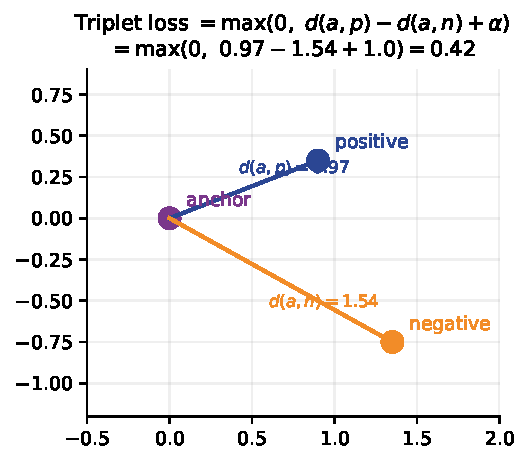
\includegraphics[width=\textwidth]{triplet.pdf}
    \end{column}
  \end{columns}
\end{frame}

\begin{frame}{Most triplets teach you nothing}
  \begin{center}
    For the figure: $L = \max(0,\; 0.97 - 1.54 + 1.0) = \mathbf{0.42}$\\[0.4em]
    \small The ordering is already right, but only by $0.58$ --- short of the
    margin --- so a penalty remains.
  \end{center}
  \vspace{0.8em}
  \begin{alertblock}{Triplet mining}
    Pick three examples at random and the constraint is usually \emph{already
    satisfied}: zero loss, zero gradient, nothing learned.\\[0.4em]
    Real systems spend most of their engineering effort hunting the hard cases
    where $d(a,p)$ is nearly as large as $d(a,n)$. Without mining, training
    stalls almost immediately.
  \end{alertblock}
\end{frame}

% =====================================================================
\section{Choosing a loss}
\label{sec:choose}

\begin{frame}[shrink=8]{A decision table}
  \begin{center}\small
  \begin{tabular}{@{}p{4.4cm}p{2.9cm}p{5.6cm}@{}}
    \toprule
    \textbf{Situation} & \textbf{Use} & \textbf{Because}\\
    \midrule
    Regression, clean, symmetric errors & MSE & smooth, fast; the mean is the sensible target\\[2pt]
    Regression, outliers you distrust & MAE & fits the typical case\\[2pt]
    Regression, outliers you cannot exclude & Huber & quadratic where it matters, linear where it would distort\\[2pt]
    Two classes, want probabilities & Binary cross-entropy & calibrated; punishes confident errors\\[2pt]
    $K$ classes, one-hot labels & Categorical CE & same loss, one-hot API\\[2pt]
    $K$ classes, integer labels & Sparse categorical CE & same loss, far less memory\\[2pt]
    Two classes, want a wide boundary & Hinge & ignores points already safely correct\\[2pt]
    Embedding where similar = close & Triplet & relative distance; handles unseen identities\\
    \bottomrule
  \end{tabular}
  \end{center}
\end{frame}

\begin{frame}{The mistake to avoid}
  \begin{alertblock}{Do not choose by asking which gives the smaller number}
    Losses live on different scales and are \textbf{not comparable to each
    other}.
  \end{alertblock}
  \vspace{0.5em}
  \begin{center}
    From our four houses --- \emph{identical predictions}:\\[0.4em]
    $\mathrm{MAE} = 1.0$ \qquad $\mathrm{MSE} = 1.375$\\[0.4em]
    \small MAE is not "better". They are different quantities in different
    units.
  \end{center}
  \vspace{0.6em}
  \begin{exampleblock}{The rule}
    Compare \textbf{models} using a single fixed metric on held-out data.\\
    Use the loss to \emph{train}; use the metric to \emph{decide}.
  \end{exampleblock}
\end{frame}

% =====================================================================
\section{Summary}
\label{sec:summary}

\begin{frame}[shrink=5]{Summary}
  \begin{enumerate}\small
    \item A loss compresses mistakes into one number; that choice declares
      what kind of mistake you consider serious.
    \item Loss, cost and metric are three different things.
    \item \textbf{MSE fits the mean, MAE fits the median.} One outlier moved
      our MSE constant from $12.33$ to $25.67$ and left MAE untouched.
    \item Huber is MSE near zero and MAE far away. $\delta$ carries the units
      of $y$.
    \item Accuracy cannot be a training loss --- step function, zero gradient.
      We minimise smooth surrogates.
    \item Cross-entropy $= -\log$ (probability given to the correct class).
      Confident and wrong is unboundedly expensive.
    \item Categorical and sparse categorical are the \emph{same loss},
      different label format.
    \item Hinge charges nothing beyond margin 1 --- hence support vectors.
    \item Triplet loss trains on relative distance and needs hard mining.
  \end{enumerate}
\end{frame}

\begin{frame}[shrink=3]{Before the next lecture}
  \begin{columns}[T]
    \begin{column}{0.48\textwidth}
      \begin{block}{Read}
        \texttt{notes.pdf} --- full derivations, the median proof, and
        \textbf{10 practice questions with worked solutions}.
      \end{block}
      \begin{block}{Do}
        Questions 2, 4 and 10. Question 10 ties the whole lecture together.
      \end{block}
    \end{column}
    \begin{column}{0.48\textwidth}
      \begin{exampleblock}{Next: Unit III --- Optimizers}
        We now know \emph{what} to minimise.\\[0.3em]
        Next: gradient descent, mini-batches and momentum --- \emph{how} the
        minimising actually happens.
      \end{exampleblock}
    \end{column}
  \end{columns}
  \begin{center}
    \small Materials: \texttt{\AMLRepoURL}
  \end{center}
  \slidesources{\AMLUnitIISources}
\end{frame}

\end{document}
